\clearpage
\section{Prospective Reference-Branch Figures}

\begin{figure}[!ht]
\centering
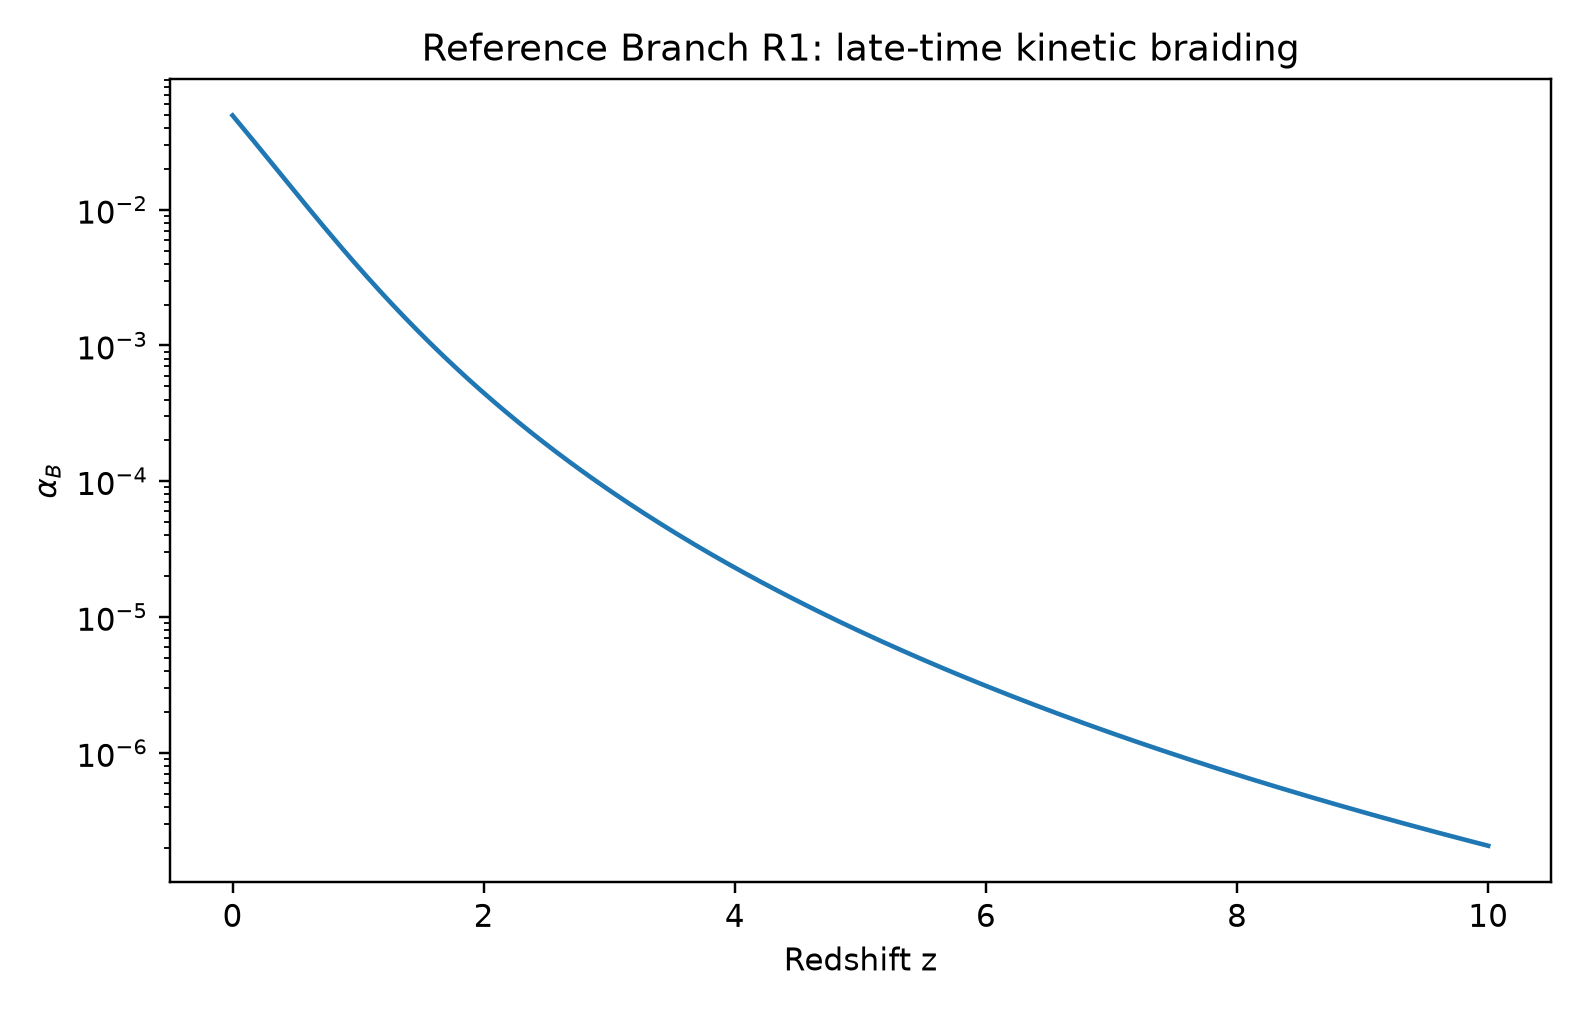
\includegraphics[width=0.68\linewidth]{figures/r1_alphaB.png}
\caption{Conditional reference calculation, not an observational fit: kinetic-braiding function \(\alpha_B(z)\) for Reference Branch R1. The logarithmic vertical scale emphasizes the suppression of the braiding sector toward high redshift.}
\label{fig:r1alphab}
\end{figure}


\begin{figure}[!ht]
\centering
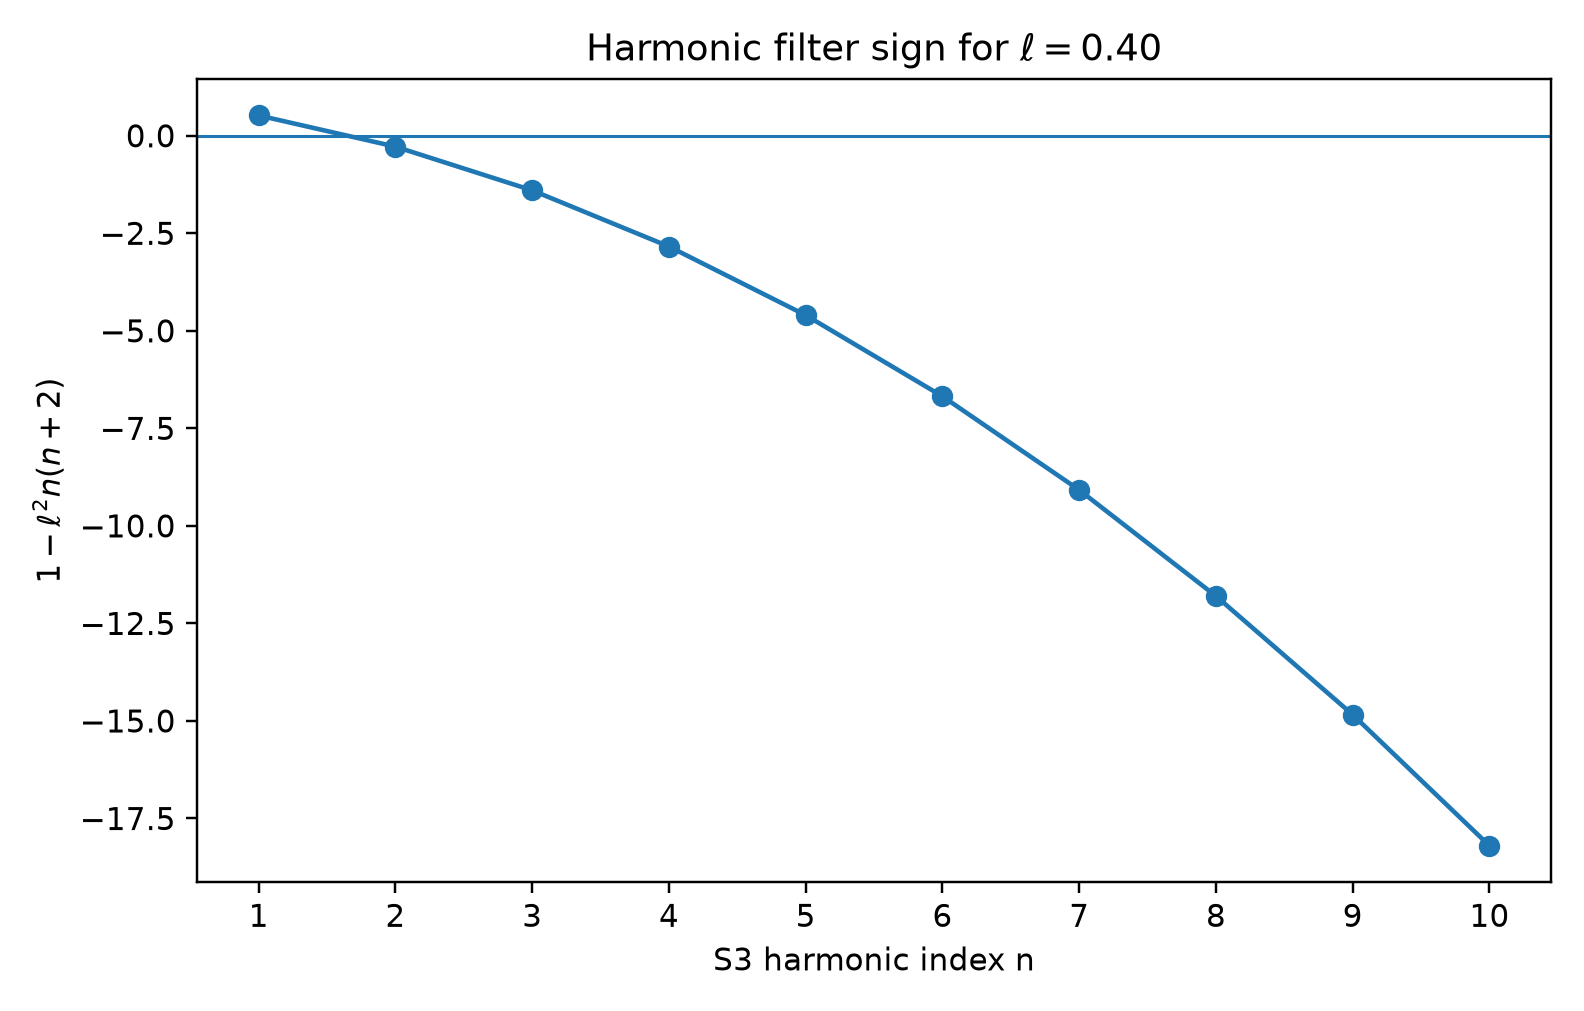
\includegraphics[width=0.68\linewidth]{figures/harmonic_filter.png}
\caption{Sign of the Schur-response factor \(1-\ell^2 n(n+2)\) for the illustrative filtering value \(\ell=0.32\), matching the canonical code. The physical \(n=2\) branch is softened and \(n\ge3\) stiffened; the displayed \(n=1\) coefficient is exceptional and excluded from propagation.}
\label{fig:harmonicfilter}
\end{figure}
